\documentclass[11pt]{article}

% packages
\usepackage{enumerate}
\usepackage{fancyhdr}
\usepackage{extramarks}
\usepackage{amsmath}
\usepackage{amsthm}
\usepackage{amssymb}
%\usepackage{amsfonts}
\usepackage{tikz}
\usepackage[plain]{algorithm}
\usepackage{algpseudocode}
\usepackage{lastpage}
\usepackage{units}
\usepackage[margin=0.75in]{geometry}
\usepackage{pgfplots}
\pgfplotsset{compat=1.16}
\usepackage{sectsty}
\usepackage{hyperref}
\usepackage{multicol}
\usepackage{mathtools}
\usepackage{tikz}
\usetikzlibrary{matrix}
\usepackage{listings}
\usepackage[plain]{algorithm}
\usepackage{algpseudocode}
\usepackage{mdframed}
\usepackage{booktabs}

\definecolor{sblue}{HTML}{5292c0}
\definecolor{sgreen}{HTML}{93c47d}
\definecolor{sorange}{HTML}{e69138}
\definecolor{codeblue}{rgb}{0.29296875, 0.51953125, 0.68359375}
\definecolor{codegreen}{rgb}{0.47265625, 0.62890625, 0.40234375}
\definecolor{codegray}{rgb}{0.95703125, 0.95703125, 0.95703125}
\definecolor{codecrimson}{rgb}{0.87109375,0.3984375,0.3984375}

\lstset{frame=tb,
  backgroundcolor=\color{codegray},
  aboveskip=3mm,
  belowskip=3mm,
  showstringspaces=false,
  columns=flexible,
  basicstyle={\small\ttfamily},
  numbers=left,
  numberstyle=\tiny\color{gray},
  keywordstyle=\color{codeblue},
  commentstyle=\color{codegreen},
  stringstyle=\color{codecrimson},
  breaklines=true,
  breakatwhitespace=true,
  tabsize=4,
  frame=tlbr,framesep=4pt,framerule=0pt,
  literate={`}{\`}1,
}

% colors
\definecolor{sblue}{HTML}{5292c0}
\definecolor{sgreen}{HTML}{93c47d}
\definecolor{sorange}{HTML}{e69138}

% sectioning magic
\counterwithin*{equation}{section}
%\numberwithin{equation}{section}

% fonts
\usepackage{fontspec}
\newfontfamily\headerfontlt{ITC Franklin Gothic Std Book}
\newfontfamily\headerfont{ITC Franklin Gothic Std Demi}
\usepackage[urw-garamond]{mathdesign}
\usepackage{garamondx}
\usepackage[italic]{mathastext}

\newcommand{\printsection}[1]{\normalfont\headerfontlt{{{#1}}}}
\newcommand{\printsubsection}[1]{\normalfont\headerfontlt\textcolor{darkgray}{{#1}}}
\newcommand{\printsubsubsection}[1]{\normalfont\headerfontlt{{#1}}}
\allsectionsfont{\printsection}
\subsectionfont{\printsection}
\subsectionfont{\printsubsection}
\subsubsectionfont{\printsubsubsection}


\renewcommand{\headrulewidth}{0.1pt}
\renewcommand{\headrule}{\hbox to\headwidth{\color{gray}\leaders\hrule height \headrulewidth\hfill}}
\renewcommand{\footrulewidth}{0.0pt}

\newcommand{\op}[1]{\textrm{\small\printsubsection{\MakeUppercase{#1}}}\,}
\newcommand{\opns}[1]{\textrm{\small\printsubsection{\MakeUppercase{#1}}}}
\newcommand{\Partial}[1]{\partial\hspace{-0.2ex}{#1}}
\newcommand{\D}[1]{\mathrm{d}#1}
\newcommand{\E}[1]{\mathbb{E}{\left[\,#1\,\right]}}
\newcommand{\var}[1]{\mathrm{var}\left( #1 \right)}
\newcommand{\cov}[1]{\mathrm{cov}\left( #1 \right)}
\newcommand{\pr}[1]{\mathrm{Pr}\left( #1 \right)}
\newcommand{\given}{\,|\,}
\renewcommand{\det}{\mathrm{det\,}}
\renewcommand{\det}[1]{\op{det}\left(#1\right)}
\renewcommand{\ker}{\mathrm{Ker\,}}
\newcommand{\trace}[1]{\op{trace}\left(#1\right)}
\newcommand{\nul}[1]{\op{nul}\left(#1\right)}
\newcommand{\col}[1]{\op{col}\left(#1\right)}
\newcommand{\row}[1]{\op{row}\left(#1\right)}
\newcommand{\rank}[1]{\op{rank}\left(#1\right)}
\renewcommand{\dim}[1]{\op{dim}\left(#1\right)}
\newcommand{\im}{\op{Im\,}}
\newcommand{\reals}{\mathbb{R}}
\newcommand{\complex}{\mathbb{C}}
\renewcommand{\vec}[1]{\mathbf{#1}}
\newcommand*{\matr}[1]{\mathbfit{#1}}
\newcommand*{\tran}{^{\mkern-1.5mu\mathsf{T}}}
\newcommand*{\conj}[1]{\overline{#1}}
\newcommand*{\hermconj}{^{\mathsf{H}}}
\newcommand*{\inv}{^{-1}}

\setlength\parindent{0pt}
\pagecolor{gray!1}


% header/footer
\topmargin=-0.65in
\pagestyle{fancy}\fancyhf{} 
\lhead{\headerfontlt{\textcolor{darkgray}{Satej Soman \textcolor{gray}{$\big/$} CAPP30254, Spring 19 \textcolor{gray}{$\big/$}} Homework 2}}
\rhead{\headerfontlt{\textcolor{gray}{$\big[$} \thepage\ \textcolor{gray}{$\big/$} \pageref{LastPage} \textcolor{gray}{$\big]$}}}

\begin{document}
\begin{titlepage}
\raggedleft\huge\headerfontlt{
\textcolor{darkgray}{Satej Soman\\
CAPP30254: Machine Learning for Public Policy\\
Spring 2019}}

\vspace{240pt}
\Huge\headerfontlt{\textcolor{darkgray}{HW 2\\MACHINE LEARNING PIPELINE}}
\vfill
\normalfont \normalsize
\tableofcontents

\end{titlepage}
\section*{Notes}
\begin{itemize}
\item Representative code snippets are interspersed with analysis and explanations below; all code is available on GitHub: \url{https://github.com/satejsoman/capp30254/tree/master/hw2/code}.
\item The pipeline library lives in the \texttt{code/pipeline} directory, while the sample application which imports the library is \texttt{code/distress-classifier.py}.
\end{itemize}

\section{Pipeline Library Design}
\subsection{Overview}
The \texttt{pipeline} library is a Python utility for declaratively creating sequences of data transformations and machine learning test/training routines. The two main classes are: 

\begin{itemize}
\item \texttt{Pipeline}, which specifies input data sources, output directories, transformation sequences, and machine learning model parameters.
\item \texttt{Transformation}, a wrapper over a Python callable, annotated with a human-readable name, and a declaration of input and output columns. In implementation, there is no difference between generating new columns in data cleaning/processing and generating feature vectors, so both stages are represented by collections of \texttt{Transformation} objects. 
\end{itemize}
\subsection{Design Decisions}
The \texttt{pipeline} library aims for:
\begin{itemize}
\item \textbf{reproducibility}: each pipeline run logs transformation steps, model parameters, pipeline library version, and input data hashes in order to create uniquely identifiable output artifacts. 
\item \textbf{debuggability}: each step is logged to \texttt{stdout} and a persistent file in a human readable manner so end users can understand the state of the pipeline. 
\item \textbf{customization}: the declarative syntax for \texttt{Pipeline} objects is flexible enough to chain machine learning pipelines or include multiple stages of preprocessing and feature generation.
\end{itemize}

To a large extent, \texttt{Pipeline} is a wrapper over on Pandas \texttt{DataFrame} objects. 
\subsection{Extensibility}
To customize functionality, the \texttt{Pipeline} class can be subclassed, or individual \texttt{Pipeline} instance can have bound methods replaced by application-level code (e.g. "monkey-patching"). The example application in section 2 uses the latter approach. 

Additionally, by rigorously tracking transformation sequences, input data, and model parameters, the library is, in principle, able to support caching of steps (i.e. no need to recompute features if they have not changed), though this feature has not been implemented at time of writing.

\pagebreak
\section{Application of ML Pipeline to Financial Distress Prediction}
\subsection{Background}
When making a decision on whether to lend to an individual, banks and financial institutions have access to a number of demographic and financial variables for each prospective borrower. The lenders would like to know, at decision time, the risk that a loan will not be repaid. With historical financial delinquency information and the \texttt{pipeline} library, we can use these demographic and financial data to build a model to predict whether a person is a serious risk for non-repayment of a loan.

\subsection{Summary Statistics}
In order to generate the summary statistics, we can write a custom summary function and attach it to our pipeline:

\begin{lstlisting}[language=Python, numbers=none]
from types import MethodType

def summarize_fd_data(self):
    self.logger.info("Running custom summary function")
    df = self.dataframe
    summary = (df
        .describe(percentiles=[])
        .drop("count")
        .drop("50%")
        .append(pd.DataFrame(
            [df.corr()[self.target].apply(np.abs), df.isnull().sum()], 
            index=["abs corr", "missing"]))
        .T
        .rename(dict(zip(summary.index, clean_names))
        .sort_values("abs corr", ascending=False))

    with (self.output_dir/"summary.tex").open('w') as fer:
        summary.to_latex(buf=fer, float_format="%.2f")

    for column in df.columns, colors:
        df[[column]].plot.hist(bins=20)
        matplotlib2tikz.save(self.output_dir/(column + ".tex"), figureheight="3in", figurewidth="3in")
    return self


pipeline = Pipeline(...)
pipeline.summarize_data = MethodType(summarize_fd_data, pipeline)

\end{lstlisting}
\begin{table}[H]
\centering \renewcommand{\arraystretch}{1.2}
\begin{tabular}{lrrrrrr}
\toprule
{} &      mean &      std &      min &        max &  abs corr &  missing \\
\midrule
delinquency                 &      0.16 &     0.37 &     0.00 &       1.00 &      1.00 &     0.00 \\
id                          & 115800.15 & 28112.72 &    22.00 &  149999.00 &      0.62 &     0.00 \\
age                         &     51.68 &    14.75 &    21.00 &     109.00 &      0.17 &     0.00 \\
payments 30-59 days late    &      0.59 &     5.21 &     0.00 &      98.00 &      0.15 &     0.00 \\
payments 90 days late       &      0.42 &     5.19 &     0.00 &      98.00 &      0.14 &     0.00 \\
payments 60-89 days late    &      0.37 &     5.17 &     0.00 &      98.00 &      0.12 &     0.00 \\
number of dependents        &      0.77 &     1.12 &     0.00 &      13.00 &      0.07 &  1037.00 \\
zipcode                     &  60623.82 &    11.98 & 60601.00 &   60644.00 &      0.05 &     0.00 \\
number of credit lines      &      8.40 &     5.21 &     0.00 &      56.00 &      0.04 &     0.00 \\
monthly income              &   6579.00 & 13446.83 &     0.00 & 1794060.00 &      0.03 &  7974.00 \\
debt ratio                  &    331.46 &  1296.11 &     0.00 &  106885.00 &      0.01 &     0.00 \\
number of real estate loans &      1.01 &     1.15 &     0.00 &      32.00 &      0.01 &     0.00 \\
revolving utilization       &      6.38 &   221.62 &     0.00 &   22000.00 &      0.00 &     0.00 \\
\bottomrule
\end{tabular}

\caption{Table of relevant summary statistics.}\label{summary}
\end{table}

The following figures show the distributions of some sample variables:

\begin{minipage}{0.45\textwidth}
\vspace{10.5pt}
\begin{figure}[H]
% This file was created by matplotlib2tikz v0.7.4.
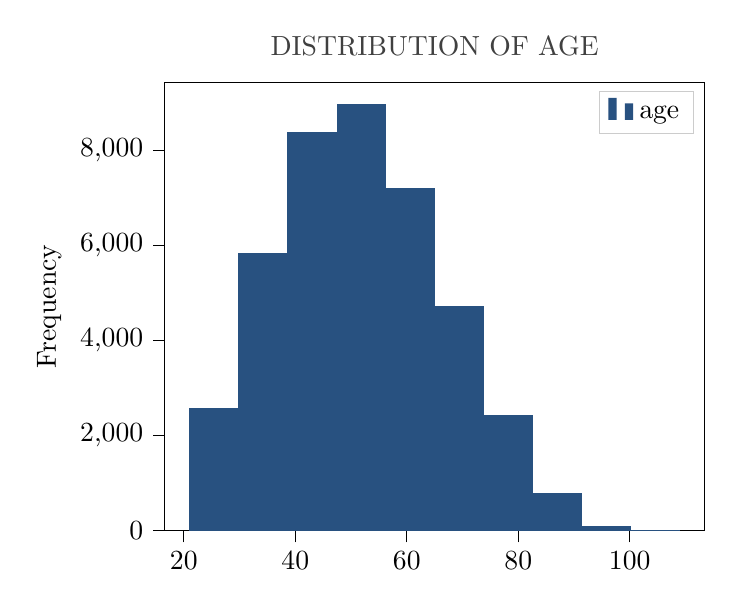
\begin{tikzpicture}

\definecolor{color0}{rgb}{0.156862745098039,0.317647058823529,0.501960784313725}

\begin{axis}[
legend cell align={left},
legend style={draw=white!80.0!black},
tick align=outside,
tick pos=left,
title={\printsubsection{\MakeUppercase{Distribution of age}}},
x grid style={white!69.01960784313725!black},
xmin=16.6, xmax=113.4,
xtick style={color=black},
y grid style={white!69.01960784313725!black},
ylabel={Frequency},
ymin=0, ymax=9433.2,
ytick style={color=black}
]
\draw[fill=color0,draw opacity=0] (axis cs:21,0) rectangle (axis cs:29.8,2585);
\addlegendimage{ybar,ybar legend,fill=color0,draw opacity=0};
\addlegendentry{age}

\draw[fill=color0,draw opacity=0] (axis cs:29.8,0) rectangle (axis cs:38.6,5834);
\draw[fill=color0,draw opacity=0] (axis cs:38.6,0) rectangle (axis cs:47.4,8375);
\draw[fill=color0,draw opacity=0] (axis cs:47.4,0) rectangle (axis cs:56.2,8984);
\draw[fill=color0,draw opacity=0] (axis cs:56.2,0) rectangle (axis cs:65,7197);
\draw[fill=color0,draw opacity=0] (axis cs:65,0) rectangle (axis cs:73.8,4724);
\draw[fill=color0,draw opacity=0] (axis cs:73.8,0) rectangle (axis cs:82.6,2436);
\draw[fill=color0,draw opacity=0] (axis cs:82.6,0) rectangle (axis cs:91.4,793);
\draw[fill=color0,draw opacity=0] (axis cs:91.4,0) rectangle (axis cs:100.2,86);
\draw[fill=color0,draw opacity=0] (axis cs:100.2,0) rectangle (axis cs:109,2);
\end{axis}

\end{tikzpicture}
\vspace{5pt}
\caption{Distribution of \texttt{age}}
\end{figure}
\end{minipage}\hfill
\begin{minipage}{0.45\textwidth}
\vspace{0pt}
\begin{figure}[H]
% This file was created by matplotlib2tikz v0.7.4.
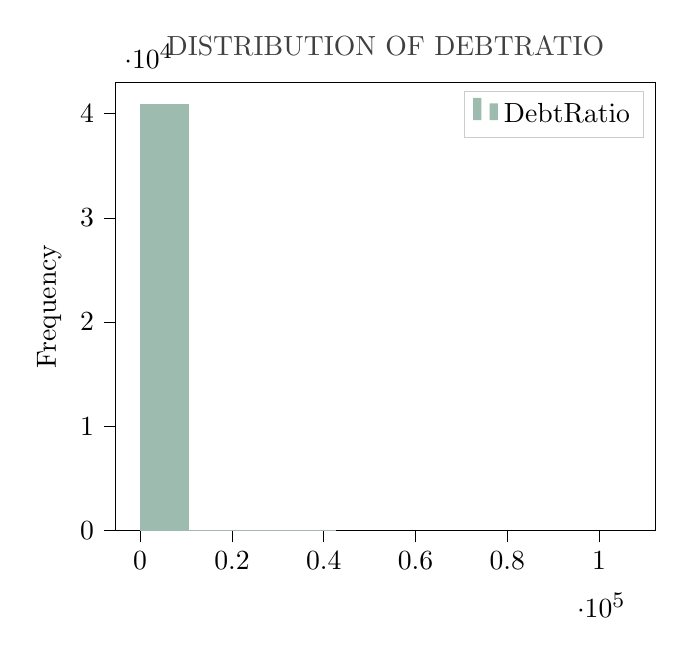
\begin{tikzpicture}

\definecolor{color0}{rgb}{0.615686274509804,0.733333333333333,0.682352941176471}

\begin{axis}[
legend cell align={left},
legend style={draw=white!80.0!black},
tick align=outside,
tick pos=left,
title={\printsubsection{\MakeUppercase{Distribution of DebtRatio}}},
x grid style={white!69.01960784313725!black},
xmin=-5344.25, xmax=112229.25,
xtick style={color=black},
y grid style={white!69.01960784313725!black},
ylabel={Frequency},
ymin=0, ymax=43016.4,
ytick style={color=black}
]
\draw[fill=color0,draw opacity=0] (axis cs:0,0) rectangle (axis cs:10688.5,40968);
\addlegendimage{ybar,ybar legend,fill=color0,draw opacity=0};
\addlegendentry{DebtRatio}

\draw[fill=color0,draw opacity=0] (axis cs:10688.5,0) rectangle (axis cs:21377,36);
\draw[fill=color0,draw opacity=0] (axis cs:21377,0) rectangle (axis cs:32065.5,6);
\draw[fill=color0,draw opacity=0] (axis cs:32065.5,0) rectangle (axis cs:42754,3);
\draw[fill=color0,draw opacity=0] (axis cs:42754,0) rectangle (axis cs:53442.5,1);
\draw[fill=color0,draw opacity=0] (axis cs:53442.5,0) rectangle (axis cs:64131,1);
\draw[fill=color0,draw opacity=0] (axis cs:64131,0) rectangle (axis cs:74819.5,0);
\draw[fill=color0,draw opacity=0] (axis cs:74819.5,0) rectangle (axis cs:85508,0);
\draw[fill=color0,draw opacity=0] (axis cs:85508,0) rectangle (axis cs:96196.5,0);
\draw[fill=color0,draw opacity=0] (axis cs:96196.5,0) rectangle (axis cs:106885,1);
\end{axis}

\end{tikzpicture}
\caption{Distribution of \texttt{DebtRatio}}
\end{figure}
\end{minipage}

\begin{minipage}[t]{0.45\textwidth}
\vspace{0pt}
\begin{figure}[H]
% This file was created by matplotlib2tikz v0.7.4.
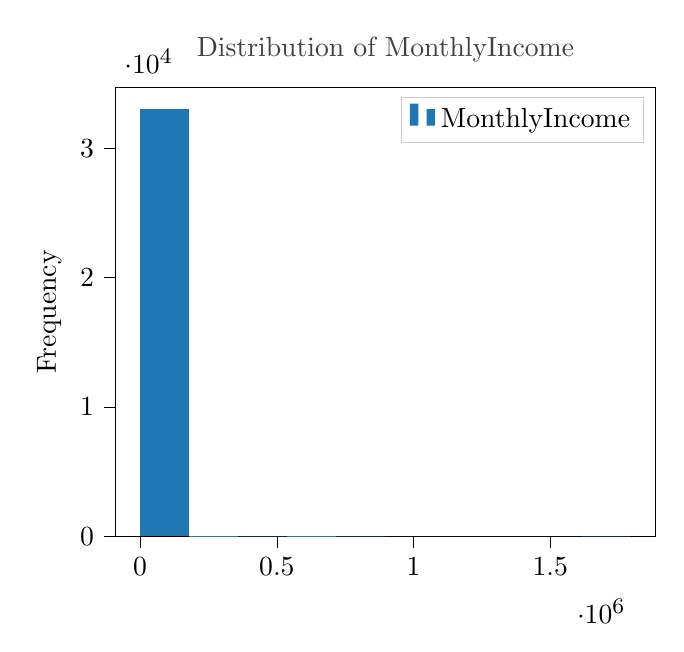
\begin{tikzpicture}

\definecolor{color0}{rgb}{0.12156862745098,0.466666666666667,0.705882352941177}

\begin{axis}[
legend cell align={left},
legend style={draw=white!80.0!black},
tick align=outside,
tick pos=left,
title={\printsubsection{Distribution of MonthlyIncome}},
x grid style={white!69.01960784313725!black},
xmin=-89703, xmax=1883763,
xtick style={color=black},
y grid style={white!69.01960784313725!black},
ylabel={Frequency},
ymin=0, ymax=34684.65,
ytick style={color=black}
]
\draw[fill=color0,draw opacity=0] (axis cs:0,0) rectangle (axis cs:179406,33033);
\addlegendimage{ybar,ybar legend,fill=color0,draw opacity=0};
\addlegendentry{MonthlyIncome}

\draw[fill=color0,draw opacity=0] (axis cs:179406,0) rectangle (axis cs:358812,4);
\draw[fill=color0,draw opacity=0] (axis cs:358812,0) rectangle (axis cs:538218,1);
\draw[fill=color0,draw opacity=0] (axis cs:538218,0) rectangle (axis cs:717624,2);
\draw[fill=color0,draw opacity=0] (axis cs:717624,0) rectangle (axis cs:897030,1);
\draw[fill=color0,draw opacity=0] (axis cs:897030,0) rectangle (axis cs:1076436,0);
\draw[fill=color0,draw opacity=0] (axis cs:1076436,0) rectangle (axis cs:1255842,0);
\draw[fill=color0,draw opacity=0] (axis cs:1255842,0) rectangle (axis cs:1435248,0);
\draw[fill=color0,draw opacity=0] (axis cs:1435248,0) rectangle (axis cs:1614654,0);
\draw[fill=color0,draw opacity=0] (axis cs:1614654,0) rectangle (axis cs:1794060,1);
\end{axis}

\end{tikzpicture}
\caption{Distribution of \texttt{MonthlyIncome}}
\end{figure}
\end{minipage}\hfill
\begin{minipage}[t]{0.45\textwidth}
\vspace{0pt}
\begin{figure}[H]
% This file was created by matplotlib2tikz v0.7.4.
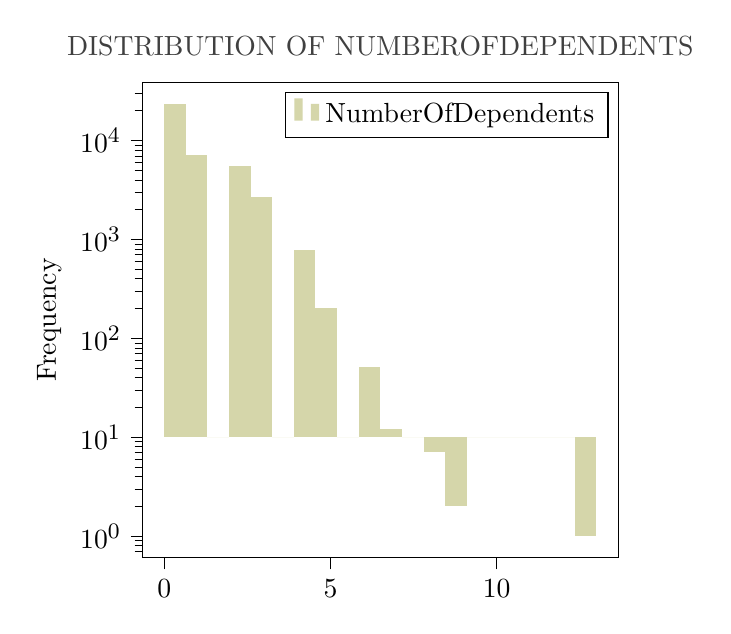
\begin{tikzpicture}

\definecolor{color0}{rgb}{0.835294117647059,0.83921568627451,0.666666666666667}

\begin{axis}[
height=3in,
log basis y={10},
tick align=outside,
tick pos=left,
title={\printsubsection{\MakeUppercase{Distribution of NumberOfDependents}}\\},
width=3in,
x grid style={white!69.01960784313725!black},
xmin=-0.65, xmax=13.65,
xtick style={color=black},
y grid style={white!69.01960784313725!black},
ylabel={Frequency},
ymin=0.604566160915982, ymax=38875.8113163171,
ymode=log,
ytick style={color=black}
]
\draw[fill=color0,draw opacity=0] (axis cs:0,0) rectangle (axis cs:0.65,23503);
\addlegendimage{ybar,ybar legend,fill=color0,draw opacity=0};
\addlegendentry{NumberOfDependents}

\draw[fill=color0,draw opacity=0] (axis cs:0.65,0) rectangle (axis cs:1.3,7211);
\draw[fill=color0,draw opacity=0] (axis cs:1.3,0) rectangle (axis cs:1.95,0);
\draw[fill=color0,draw opacity=0] (axis cs:1.95,0) rectangle (axis cs:2.6,5539);
\draw[fill=color0,draw opacity=0] (axis cs:2.6,0) rectangle (axis cs:3.25,2666);
\draw[fill=color0,draw opacity=0] (axis cs:3.25,0) rectangle (axis cs:3.9,0);
\draw[fill=color0,draw opacity=0] (axis cs:3.9,0) rectangle (axis cs:4.55,786);
\draw[fill=color0,draw opacity=0] (axis cs:4.55,0) rectangle (axis cs:5.2,201);
\draw[fill=color0,draw opacity=0] (axis cs:5.2,0) rectangle (axis cs:5.85,0);
\draw[fill=color0,draw opacity=0] (axis cs:5.85,0) rectangle (axis cs:6.5,51);
\draw[fill=color0,draw opacity=0] (axis cs:6.5,0) rectangle (axis cs:7.15,12);
\draw[fill=color0,draw opacity=0] (axis cs:7.15,0) rectangle (axis cs:7.8,0);
\draw[fill=color0,draw opacity=0] (axis cs:7.8,0) rectangle (axis cs:8.45,7);
\draw[fill=color0,draw opacity=0] (axis cs:8.45,0) rectangle (axis cs:9.1,2);
\draw[fill=color0,draw opacity=0] (axis cs:9.1,0) rectangle (axis cs:9.75,0);
\draw[fill=color0,draw opacity=0] (axis cs:9.75,0) rectangle (axis cs:10.4,0);
\draw[fill=color0,draw opacity=0] (axis cs:10.4,0) rectangle (axis cs:11.05,0);
\draw[fill=color0,draw opacity=0] (axis cs:11.05,0) rectangle (axis cs:11.7,0);
\draw[fill=color0,draw opacity=0] (axis cs:11.7,0) rectangle (axis cs:12.35,0);
\draw[fill=color0,draw opacity=0] (axis cs:12.35,0) rectangle (axis cs:13,1);
\end{axis}

\end{tikzpicture}
\vspace{16pt}
\caption{Distribution of \texttt{NumberOfDependents}}
\end{figure}
\end{minipage}

\subsection{Data Preparation}
As seen in Table \ref{summary}, the columns for number of dependents and monthly income have missing values. We can clean the data by replacing the missing values in these columns by the average of the non-missing values.

\begin{lstlisting}[language=Python,numbers=none]
from pipeline.transformation import replace_missing

pipeline = Pipeline(...
    data_preprocessors=[
        replace_missing("MonthlyIncome"), 
        replace_missing("NumberOfDependents")],
    ...)
\end{lstlisting}
\pagebreak
\subsection{Feature Choices}
The variables in Table \ref{summary} are sorted by their absolute correlation with delinquency ($\vert\rho_{x,y}\vert$). Since the person's ID is likely randomly assigned, its high correlation with delinquency is spurious. Looking at the next few variables, the combination of age, along with \textit{any} payments late past 30 days, show promise of explaining delinquency well. 

We can also include income in our model; standard econometrics practice is to analyze the effects of changes in logarithmic income since the income distribution tends to be skewed.

\begin{lstlisting}[language=Python,numbers=none]
from pipeline.transformation import Transformation, replace_missing

# categorical variable
age_decade = Transformation("age-decade", ["age"], "age_decade", 
    lambda col: col.apply(lambda x: 10*(x//10))
)

# binary variable
any_late_payments = Transformation("any-late-payments", ["NumberOfTime30-59DaysPastDueNotWorse", "NumberOfTime60-89DaysPastDueNotWorse", "NumberOfTimes90DaysLate"], "any_late_payments", 
    lambda cols: cols.apply(lambda x: int(np.sum(x) > 0), axis=1)
)

log_monthly_income = Transformation("log-monthly-income", ["MonthlyIncome_clean"], "log_monthly_income", 
    lambda col: col.apply(lambda x: np.log(x + 1e-10))
)

pipeline = Pipeline(...
    feature_generators=[
        age_decade,
        any_late_payments,
        log_monthly_income],
    ...)
\end{lstlisting}


\subsection{Model Choices}
A logistic regression is appropriate here: 
$$ P\left(\text{delinquency} \ \middle\vert\ \text{data}\right) = \Lambda\left(\beta_0 + \beta_1 \left(\text{any late payments} \right) + \beta_2 \left(\text{age decade} \right) + \beta_3 \cdot \op{log}\left(\text{monthly income} \right)\right) $$

$\Lambda(w)$ is the logistic function. For this application, we use the implementation found in the scikit-learn library (\texttt{sklearn.linear\_model.LogisticRegression}).

\pagebreak
\subsection{Results}
We choose accuracy as the evaluation metric since this exercise is about the pipeline rather than the technique. Running the pipeline shows:

\begin{lstlisting}[language=Python,numbers=none]
# set up pipeline
pipeline = Pipeline(input_path, "SeriousDlqin2yrs",
    summarize=True,
    data_preprocessors=[
        replace_missing("MonthlyIncome"), 
        replace_missing("NumberOfDependents")],
    feature_generators=[
        age_decade,
        any_late_payments,
        log_monthly_income],
    model=LogisticRegression(solver="lbfgs"),
    name="financial-distress-classifier", 
    output_root_dir="output")

# attach custom summary function
pipeline.summarize_data = MethodType(summarize_fd_data, pipeline)

# run pipeline
pipeline.run()
\end{lstlisting}

The relevant portion of the pipeline output is shown:

\begin{lstlisting}[numbers=none]
Running transformations for preprocessing
    Applying transformation (1/2): replace-missing-values-with-mean(MonthlyIncome) 
    ['MonthlyIncome'] -> MonthlyIncome_clean
    Applying transformation (2/2): replace-missing-values-with-mean(NumberOfDependents) 
    ['NumberOfDependents'] -> NumberOfDependents_clean


Running transformations for feature generation
    Applying transformation (1/3): age-decade 
    ['age'] -> age_decade
    Applying transformation (2/3): any-late-payments 
    ['NumberOfTime30-59DaysPastDueNotWorse', 'NumberOfTime60-89DaysPastDueNotWorse', 'NumberOfTimes90DaysLate'] -> any_late_payments
    Applying transformation (3/3): log-monthly-income 
    ['MonthlyIncome_clean'] -> log_monthly_income

Running model LogisticRegression(C=1.0, class_weight=None, dual=False, fit_intercept=True,
          intercept_scaling=1, max_iter=100, multi_class='warn',
          n_jobs=None, penalty='l2', random_state=None, solver='lbfgs',
          tol=0.0001, verbose=0, warm_start=False)
Features: ['age_decade', 'any_late_payments', 'log_monthly_income']
Fitting: SeriousDlqin2yrs
Evaluating model
Model score: 0.8415008777062609
Copying artifacts to stable path
Finished at 2019-04-18 00:18:47.284784
\end{lstlisting}

As we can see in the pipeline output, the model score accuracy is 0.8415. This is not a fantastic score, but we have a flexible framework to quickly and effectively increase the performance of the classifier.

\end{document} 
